\chapter{Analisi dei componenti}
Nel seguente capitolo viene descritta l'architettura dei componenti interni al sistema. Prima vengono presentati i componenti specificandone anche il loro livello di \textit{coesione}, poi viene utilizzato il Component Diagram per rappresentare le connessioni tra i vari componenti. Viene infine valutato il livello di accoppiamento tra i \textit{componenti}.

\section{Definizione dei componenti}

\subsection{Interfaccia base di dati}
\textbf{Motivazione.} \'E stato identificato il componente \textbf{Interfaccia base di dati} in quanto molti dei componenti necessitano di ricevere dati dal database utilizzato per salvare tutti i dati dell'applicazione.

\vspace{5mm}
\noindent
\textbf{Coesione:} livello \textbf{6} - Informazionale. 

\noindent
\underline{Spiegazione:} Il componente fornisce i dati richiesti a tutte le componenti con cui entra in contatto per permetterne il loro funzionamento.

\subsection{Visualizzatore menù principale}
\textbf{Motivazione.} Dato il \textbf{RF 2.1} e il mock-up della schermata menù (in Figura 4.4 presente nel documento D1).\\
\'E stato quindi definito il componente \textbf{Visualizzatore menù principale} in modo da gestire le richieste dell'utente di cambiare schermata. Esso si interfaccia con il componente "interfaccia basi di dati" che fornisce tutti i dati necessari e con il componente "generatore istogrammi" per realizzare gli istogrammi da visualizzare come richiesto dal \textbf{RF 2.5}.

\vspace{5mm}
\noindent
\textbf{Coesione:} livello \textbf{4} - Procedurale. 

\noindent
\underline{Spiegazione:} il componente gestisce l'intera procedura che l'utente segue per selezionare una voce dal menù principale e richiede all'interfaccia basi di dati e generatore istogrammi di fornire i dati necessari. L'utente seleziona la voce desiderata, dopodiché il database fornisce i dati richiesti.

\subsection{Interfaccia localizzazione}
\textbf{Motivazione.} Dato il \textbf{RF 2.4.3} e il \textbf{RF 2.5} il sistema deve fornire la posizione e lo storico sul numero degli animali presenti in un'area. \'E stato quindi definito il componente \textbf{Interfaccia localizzazione} con lo scopo di gestire tutti i dati ricevuti dal sistema GPS introdotto nel \textbf{Back-End 5.5}.

\vspace{5mm}
\noindent
\textbf{Coesione:} livello \textbf{7} - Funzionale. 

\noindent
\underline{Spiegazione:} il componente fornisce la posizione e il numero di animali di medio/grandi dimensioni.

\subsection{Interfaccia ottenimento dati sensori}
\textbf{Motivazione.} \'E stato definito il componente \textbf{Interfaccia ottenimento dati sensori} con lo scopo di gestire i dati ricevuti dal sistema locale di sensori presente nel \textbf{Back-End 5.1}.

\vspace{5mm}
\noindent
\textbf{Coesione:} livello \textbf{7} - Funzionale.

\noindent
\underline{Spiegazione:} il componente gestisce i dati ricevuti dai sensori locali e li fornisce all'interfaccia di calcolo probabilistico. 

\subsection{Interfaccia calcolo probabilistico}
\textbf{Motivazione.} \'E stato definito il componente \textbf{Interfaccia calcolo probabilistico} per gestire l'interazione con il sistema di calcolo probabilistico presente nel \textbf{Back-End 5.2}.

\vspace{5mm}
\noindent
\textbf{Coesione:} livello \textbf{5} - Comunicazionale.

\noindent
\underline{Spiegazione:} il componente gestisce l'interazione tra i sensori e il sistema di calcolo probabilistico e successivamente invia i dati elaborati al database.

\subsection{Elaboratore rischio}
\textbf{Motivazione.} Dato il \textbf{RF 2.3} è stato introdotto il componente \textbf{Elaboratore rischio} per gestire la necessità di stabilire il livello di allarme attuale.

\vspace{5mm}
\noindent
\textbf{Coesione:} livello \textbf{7} - Funzionale.

\noindent
\underline{Spiegazione:} il componente ricevendo come input i dati probabilizzati dalla base di dati, stabilisce il livello di allarme corrispondente e lo fornisce all'interfaccia notifiche.

\subsection{Interfaccia notifiche}
\textbf{Motivazione.} Dato il \textbf{RF 2.4} e il sistema di invio notifiche/email (\textbf{Back-End 5.4}) è stato introdotto il componente \textbf{Interfaccia notifiche} per gestire l'invio di notifiche ai vari attori del sistema.

\vspace{5mm}
\noindent
\textbf{Coesione:} livello \textbf{5} - Comunicazionale.

\noindent
\underline{Spiegazione:} il componente riceve la lista degli utenti e dei dispositivi dal database ed il livello di allarme dall'elaboratore di rischio. Invia al sistema di invio notifiche/mail questi dati per permettere di inviare le mail agli interessati. Successivamente riceve la lista dei dispositivi da notificare ed invia le notifiche adatte.

\subsection{Gestione autenticazione}
\textbf{Motivazione.} Dato il \textbf{RF 2.2} è stato introdotto il componente \textbf{Gestione autenticazione} che comunica con l'interfaccia base di dati per verificare le credenziali fornite dall'amministratore al momento del login.

\vspace{5mm}
\noindent
\textbf{Coesione:} livello \textbf{7} - Funzionale.

\noindent
\underline{Spiegazione:} il componente gestisce la funzionalità di autenticazione dell'utente all'interno dell'app.

\subsection{Generatore istogrammi}
\textbf{Motivazione.} Dato il \textbf{RF 2.5} è stato inserito il componente \textbf{Generatore istogrammi} in quanto incaricato di generare i grafici che verranno mostrati all'utente.

\vspace{5mm}
\noindent
\textbf{Coesione:} livello \textbf{7} - Funzionale.

\noindent
\underline{Spiegazione:} il componente si occupa di generare l'istogramma sulla popolazione animale richiesta dall'utente utilizzando la posizione ed il numero degli animali in un lasso di tempo forniti dal database.

\section{Tabella riassuntiva dei livelli di coesione dei componenti}
\begin{table}[ht]
    \centering
    \begin{tabular}{|l|c|c|c|c|c|c|c|}
        \hline
        \textbf{Componenti $\backslash$  Livello di coesione} & 1 & 2 & 3 & 4 & 5 & 6 & 7 \\
        \hline
        \rowcolor{Gray}
        Interfaccia base di dati & & & & & & \textbf{x} & \\
        \hline
        Visualizzatore menù principale & & & & \textbf{x} & & & \\
        \hline
        \rowcolor{Gray}
        Interfaccia localizzazione & & & & & & & \textbf{x}\\
        \hline
        Interfaccia ottenimento dati sensori & & & & & & & \textbf{x} \\
        \hline
        \rowcolor{Gray}
        Interfaccia calcolo probabilistico & & & & & \textbf{x} & & \\
        \hline
        Elaboratore rischio & & & & & & & \textbf{x} \\
        \hline
        \rowcolor{Gray}
        Interfaccia notifiche & & & & & \textbf{x} & & \\
        \hline
        Gestione autenticazione& & & & & & & \textbf{x} \\
        \hline
        \rowcolor{Gray}
        Generatore istogrammi & & & & & & & \textbf{x}\\
        \hline
    \end{tabular}
\end{table}


\section{Diagramma dei componenti}

\begin{figure}[ht]
    \centering
    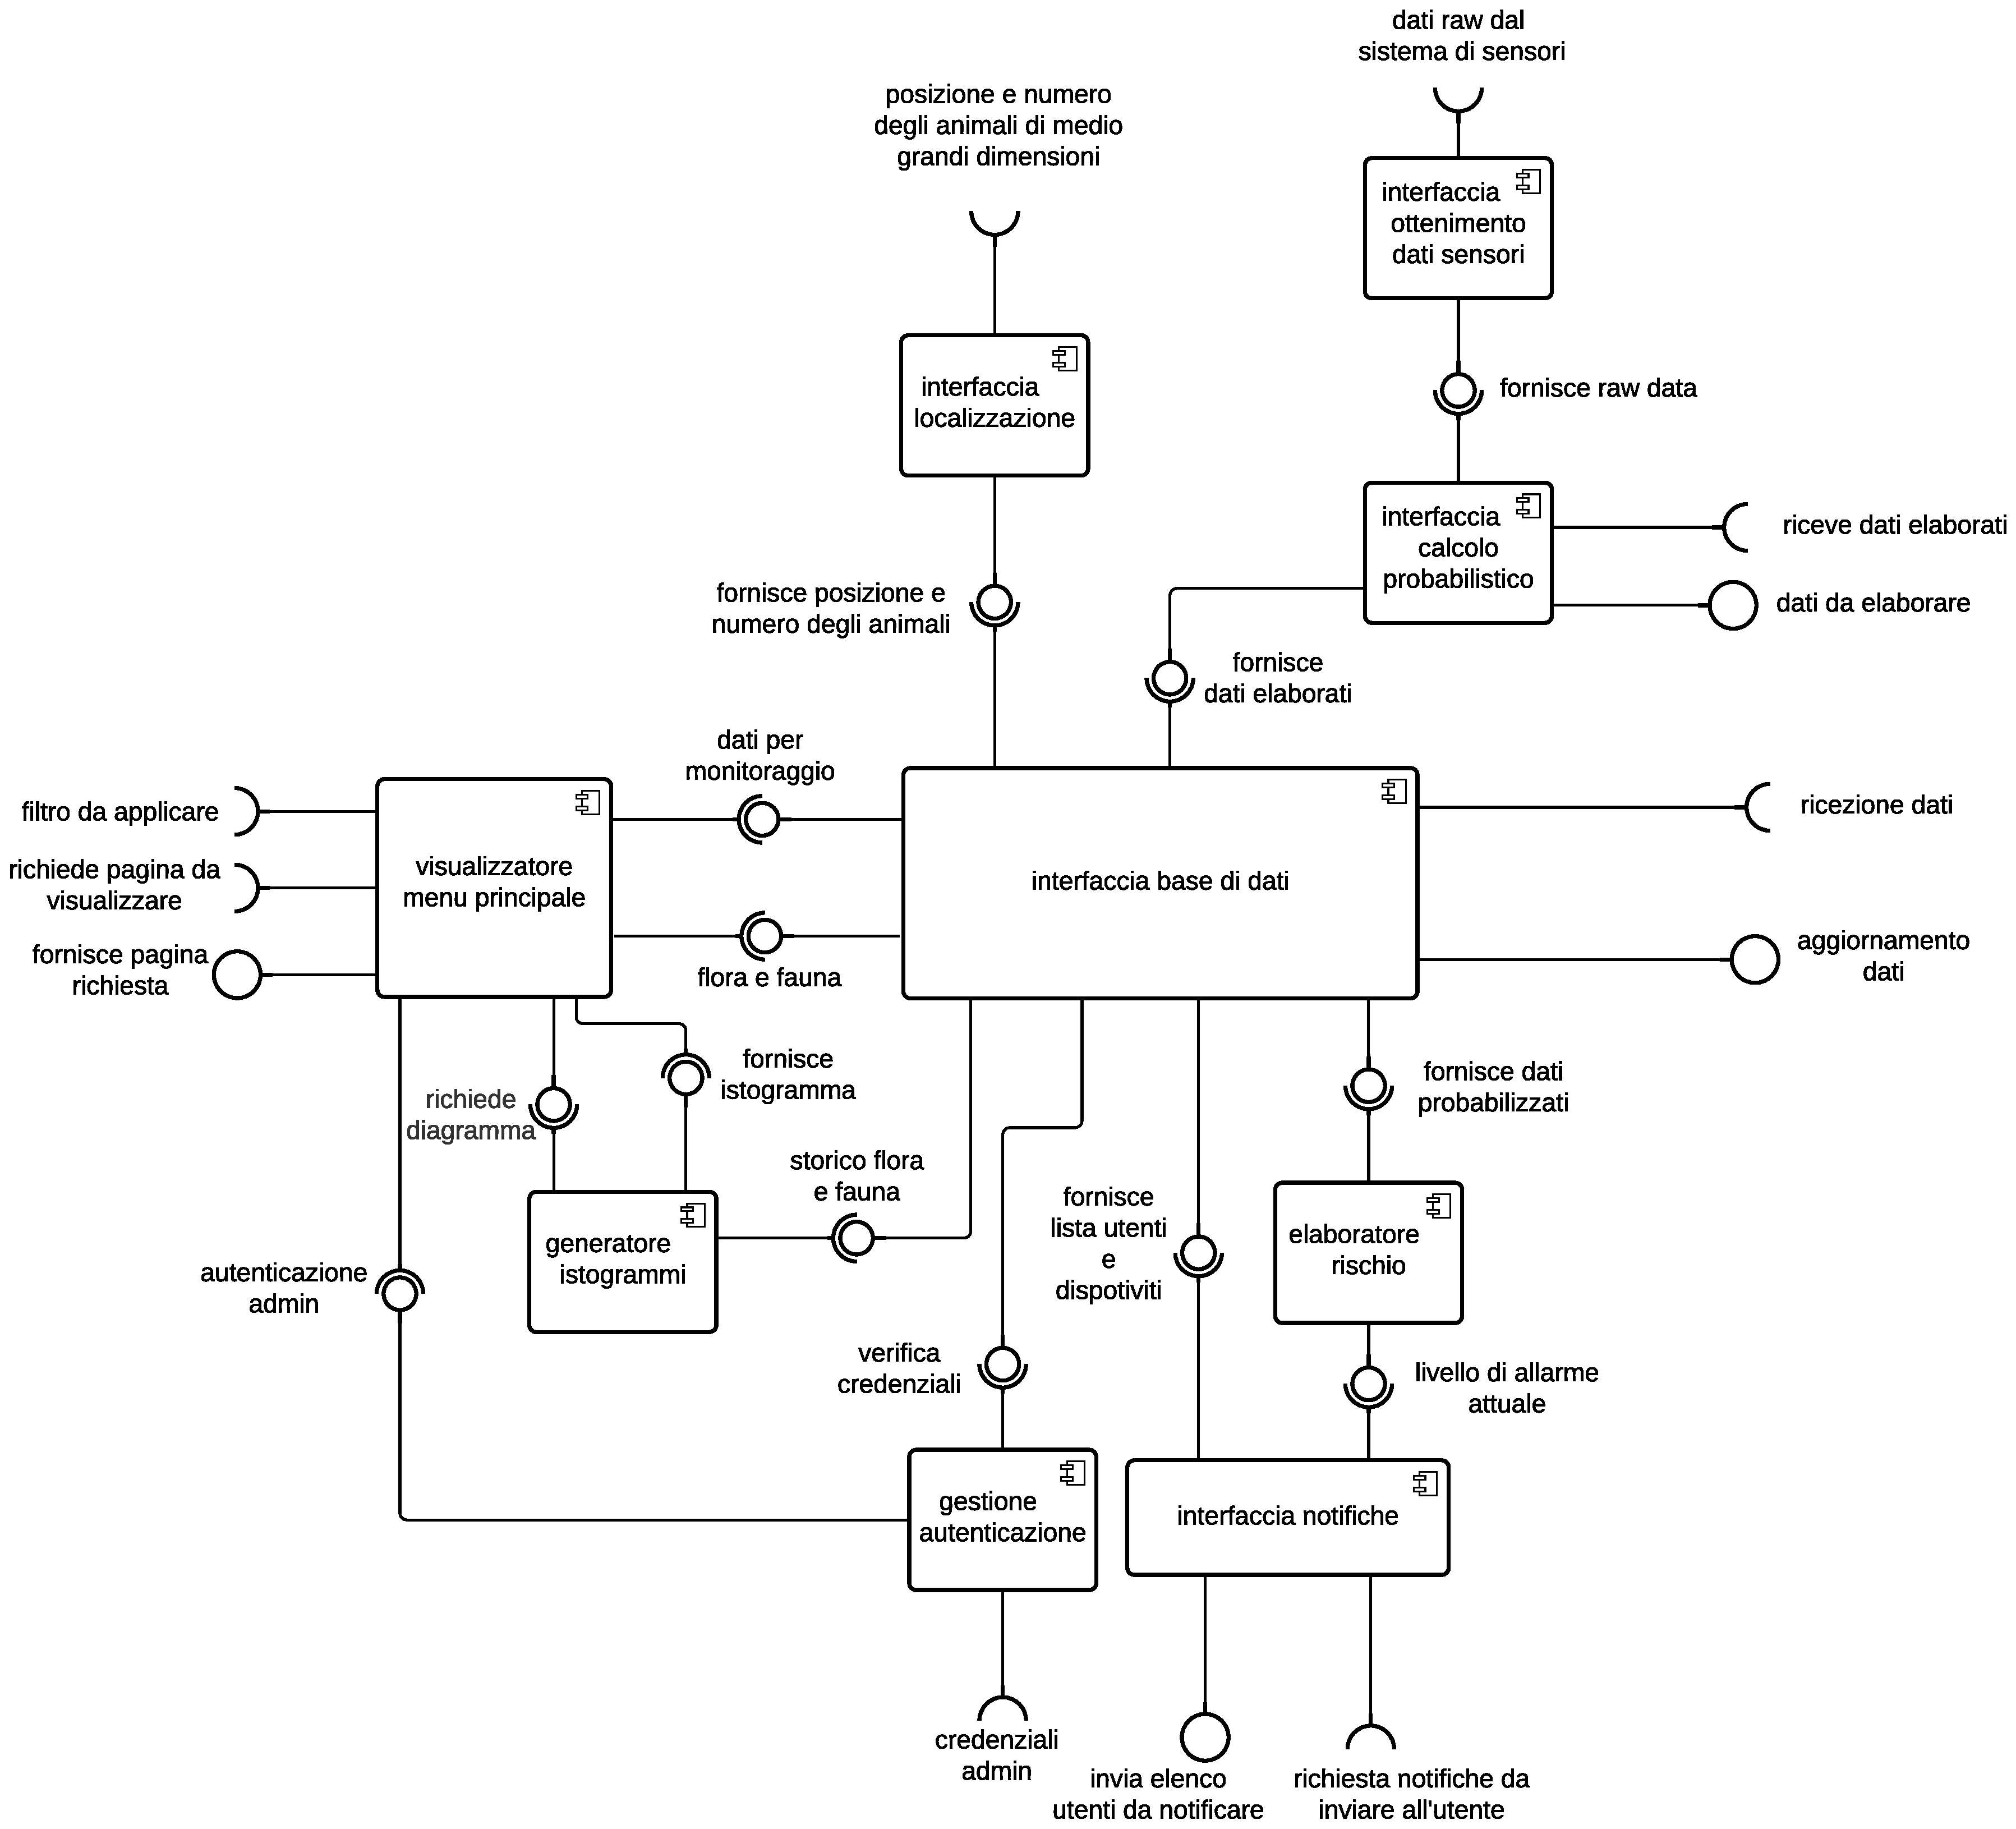
\includegraphics[scale=0.28]{Img/DiagrammaDeiComponenti.eps}
    \caption{Diagramma dei componenti per l'applicazione Sistema di monitoraggio ambientale}
\end{figure}

% ------- INTERFACCIA BASI DI DATI -------
\subsection*{Interfaccia basi di dati}
\underline{Descrizione:}
Quest'interfaccia fornisce tutti i dati necessari per far funzionare l'applicazione correttamente. Essa funziona da tramite tra il database esterno ed il sistema interno.

\vspace{5mm}
\noindent
\underline{Interfaccia richiesta - dati:}
L'interfaccia richiede e riceve i dati dal Database esterno.

\vspace{5mm}
\noindent
\underline{Interfaccia richiesta - dati elaborati:}
L'interfaccia riceve i dati elaborati dall'interfaccia di calcolo probabilistico.

\vspace{5mm}
\noindent
\underline{Interfaccia richiesta - posizione e numero animali:}
L'interfaccia riceve la posizione ed il numero degli animali dall'interfaccia di localizzazione.

\vspace{5mm}
\noindent
\underline{Interfaccia fornita - aggiornamento dati:}
L'interfaccia invia i dati ricevuti dalle altre componenti e le invia al database per aggiornarlo.

\vspace{5mm}
\noindent
\underline{Interfaccia fornita - dati probabilizzati:}
L'interfaccia fornisce all'elaboratore di rischio i dati probabilizzati calcolati precedentemente dal sistema di calcolo probabilistico.

\vspace{5mm}
\noindent
\underline{Interfaccia fornita - lista utenti e dispositivi:}
Il componente fornisce la lista di utenti e dispositivi per permettere al sistema invio notifiche/email di notificare i giusti utenti e dispositivi.

\vspace{5mm}
\noindent
\underline{Interfaccia fornita - verifica credenziali:}
Il componente fornisce i dati necessari a verificare le credenziali degli amministratori che effettuano il log-in.

\vspace{5mm}
\noindent
\underline{Interfaccia fornita - dati monitoraggio:}
L'interfaccia fornisce al visualizzatore menù principale i dati per controllare i livelli di allarme attuali nella zona. Questa richiesta può essere effettuata solo da un amministratore.

\vspace{5mm}
\noindent
\underline{Interfaccia fornita - flora e fauna:}
L'interfaccia fornisce i dati della flora e della fauna di uno specifico parco al visualizzatore menù principale.

\vspace{5mm}
\noindent
\underline{Interfaccia fornita - storico flora e fauna:}
L'interfaccia fornisce al generatore di istogrammi i dati necessari per poter creare i grafici sullo storico della popolazione. Questa richiesta può essere effettuata solo da un amministratore.

% ------- GESTISCI AUTENTICAZIONE -------
\subsection*{Gestione autenticazione}
\underline{Descrizione:} il componente si occupa della funzionalità di autenticazione tramite credenziali fornite dall'amministratore. Include la pagina per il login e il logout dell'utente e si occupa di gestire la sessione attiva.

\vspace{5mm}
\noindent
\underline{Interfaccia richiesta - credenziali admin:} le credenziali, necessarie per eseguire il login, sono username e password.

\vspace{5mm}
\noindent
\underline{Interfaccia richiesta - verifica credenziali:} la verifica delle credenziali conferma o nega l'accesso, attraverso un controllo incrociato tra i dati forniti e i dati presenti sul database.

\vspace{5mm}
\noindent
\underline{Interfaccia fornita - autenticazione admin:} la sessione dell'amministratore rimane attiva fino a quando non seleziona un'area non di sua competenza.

% ------- GENERATORE ISTOGRAMMI ------------
\subsection*{Generatore istogrammi}
\underline{Descrizione:} il componente si occupa di realizzare gli istogrammi che rappresenteranno lo storico della popolazione animale e vegetale.

\vspace{5mm}
\noindent
\underline{Interfaccia richiesta - storico flora e fauna:} Riceve la posizione e il numero degli animali nel tempo dal Database.

\vspace{5mm}
\noindent
\underline{Interfaccia richiesta - richiede diagramma:}
Il componente richiede il diagramma selezionato dall'utente nel visualizzatore menu principale.

\vspace{5mm}
\noindent
\underline{Interfaccia fornita - istogramma:} Fornisce al visualizzatore del menu gli istogrammi richiesti dall'amministratore.

% ------- INTERFACCIA LOCALIZZAZIONE -------
\subsection*{Interfaccia localizzazione}
\underline{Descrizione:} il componente si occupa di gestire i dati ricevuti dal sistema GPS. Inoltre funziona da tramite tra il sistema esterno GPS e il database.

\vspace{5mm}
\noindent
\underline{Interfaccia richiesta - posizione e numero animali:} Riceve la posizione e il numero degli animali dal sistema GPS.

\vspace{5mm}
\noindent
\underline{Interfaccia fornita - posizione e numero animali:} Fornisce all'interfaccia base di dati la posizione e il numero degli animali rilevati dal sistema GPS.

% ------- INTERFACCIA OTTENIMENTO DATI SENSORI -------
\subsection*{Interfaccia ottenimento dati sensori}
\underline{Descrizione:} il componente si occupa di gestire l'invio e la ricezione di tutti i dati rilevati dal sistema esterno "sensori".

\vspace{5mm}
\noindent
\underline{Interfaccia richiesta - dati sensori:} Riceve i dati grezzi rilevati dai sensori.

\vspace{5mm}
\noindent
\underline{Interfaccia fornita - dati sensori:} Si occupa di inviare i dati grezzi rilevati dai sensori.

% ------- INTERFACCIA CALCOLO PROBABILISTICO -------
\subsection*{Interfaccia calcolo probabilistico}
\underline{Descrizione:} il componente si occupa di gestire l'interazione tra il sistema esterno di calcolo delle probabilità e l'interfaccia base di dati.

\vspace{5mm}
\noindent
\underline{Interfaccia richiesta - raw data:} L'interfaccia riceve i dati grezzi rilevati dal sistema esterno "sensori".

\vspace{5mm}
\noindent
\underline{Interfaccia richiesta - dati elaborati:} L'interfaccia riceve i dati elaborati dal sistema esterno di calcolo delle probabilità.

\vspace{5mm}
\noindent
\underline{Interfaccia fornita - dati da elaborare:} I dati grezzi ricevuti vengono inviati al sistema esterno per trasformarli in probabilità.

\vspace{5mm}
\noindent
\underline{Interfaccia fornita - dati elaborati:} Una volta che i dati sono stati elaborati l'interfaccia si occupa di inviarli al database.

% ------- ELABORATORE RISCHIO -------
\subsection*{Elaboratore rischio}
\underline{Descrizione:} il componente si occupa di calcolare il livello di rischio basandosi sulle percentuali ricevute dal database. I valori di riferimento sono espressi nel \textbf{RF 2.3}.

\vspace{5mm}
\noindent
\underline{Interfaccia richiesta - dati probabilizzati:} I dati elaborati salvati sul database vengono ricevuti dall'elaboratore rischio che stabilirà il livello di allarme corretto.

\vspace{5mm}
\noindent
\underline{Interfaccia fornita - livello di allarme:} L'interfaccia fornisce il livello di allarme calcolato, necessario per inviare le notifiche agli attori del sistema.

% ------- INTERFACCIA NOTIFICHE -------
\subsection*{Interfaccia notifiche}
\underline{Descrizione:} il componente si occupa di gestire l'invio delle mail/notifiche agli attori del sistema: utenti, amministratori e autorità locali (la figura \ref{fig:bpmn_notifiche} descrive il funzionamento dell'invio delle notifiche ad un utente non registrato, agli amministratori ed alle autorità locali. Queste ultime due ricevono ogni modifica del livello di allarme).

\vspace{5mm}
\noindent
\underline{Interfaccia richiesta - lista utenti e dispositivi:} La lista completa degli utenti e dei dispositivi presenti nel database.

\vspace{5mm}
\noindent
\underline{Interfaccia richiesta - livello di allarme:} Il livello di allarme serve a stabilire quali utenti vanno notificati a seconda del rischio.

\vspace{5mm}
\noindent
\underline{Interfaccia richiesta - notifiche da inviare:} L'interfaccia riceve dal sistema esterno quali utenti vanno notificati solo tramite pop-up e che tipo di notifica inviare.

\vspace{5mm}
\noindent
\underline{Interfaccia fornita - elenco utenti da notificare:} L'elenco degli utenti da notificare serve al sistema esterno per sapere a chi inviare le email di allarme.

% ------- VISUALIZZATORE MENU PRINCIPALE -------
\subsection*{Visualizzatore menù principale}
\underline{Descrizione:}
Il componente si occupa dell'interazione tra l'utente e l'applicativo. Esso fornisce all'utente i dati processati da lui richiesti.

\vspace{5mm}
\noindent
\underline{Interfaccia richiesta - filtro da applicare:}
Il componente consente all'utente di applicare dei filtri sulla guida turistica. I filtri sono:
\begin{itemize}
    \item Ordinamento: alfabetico o casuale
    \item Specie: Protetta o non
    \item Popolazione: numero di esemplari (in ordine crescente/decrescente, ove possibile)
\end{itemize}

Nel caso l'utente abbia richiesto la visualizzazione di un istogramma, esso dovrà selezionare il lasso temporale desiderato tra annuale, mensile ed giornaliero.


\vspace{5mm}
\noindent
\underline{Interfaccia richiesta - richiede pagina da visualizzare:} L'interfaccia richiede all'utente di selezionare la pagina desiderata.

\vspace{5mm}
\noindent
\underline{Interfaccia richiesta - autenticazione admin:}
Nel caso l'utente voglia effettuare il login come amministratore, l'interfaccia richiede al componente "gestione autenticazione" di fornire l'autenticazione per poter dare accesso all'utente le funzionalità fruibili unicamente dall'amministratore, come visualizzare statistiche sugli animali.

\vspace{5mm}
\noindent
\underline{Interfaccia richiesta - dati per monitoraggio:}
L'interfaccia richiede i dati necessari per poter mostrare all'utente le percentuali sul rischio.

\vspace{5mm}
\noindent
\underline{Interfaccia richiesta - flora e fauna:}
Il componente richiede i dati sulla flora e la fauna di un determinato parco.

\vspace{5mm}
\noindent
\underline{Interfaccia richiesta - fornisce istogramma:} 
Nel caso l'amministratore desideri visualizzare l'istogramma di qualche specifico animale, il componente richiede al modulo "generatore istogrammi" di generare l'istogramma e fornirlo.

\vspace{5mm}
\noindent
\underline{Interfaccia fornita - fornisce pagina richiesta:} L'interfaccia fornisce all'utente la pagina da lui richiesta.

\vspace{5mm}
\noindent
\underline{Interfaccia fornita - richiede diagramma:} L'interfaccia fornisce il diagramma richiesto dall'utente.


\begin{figure}[ht]
    \centering
    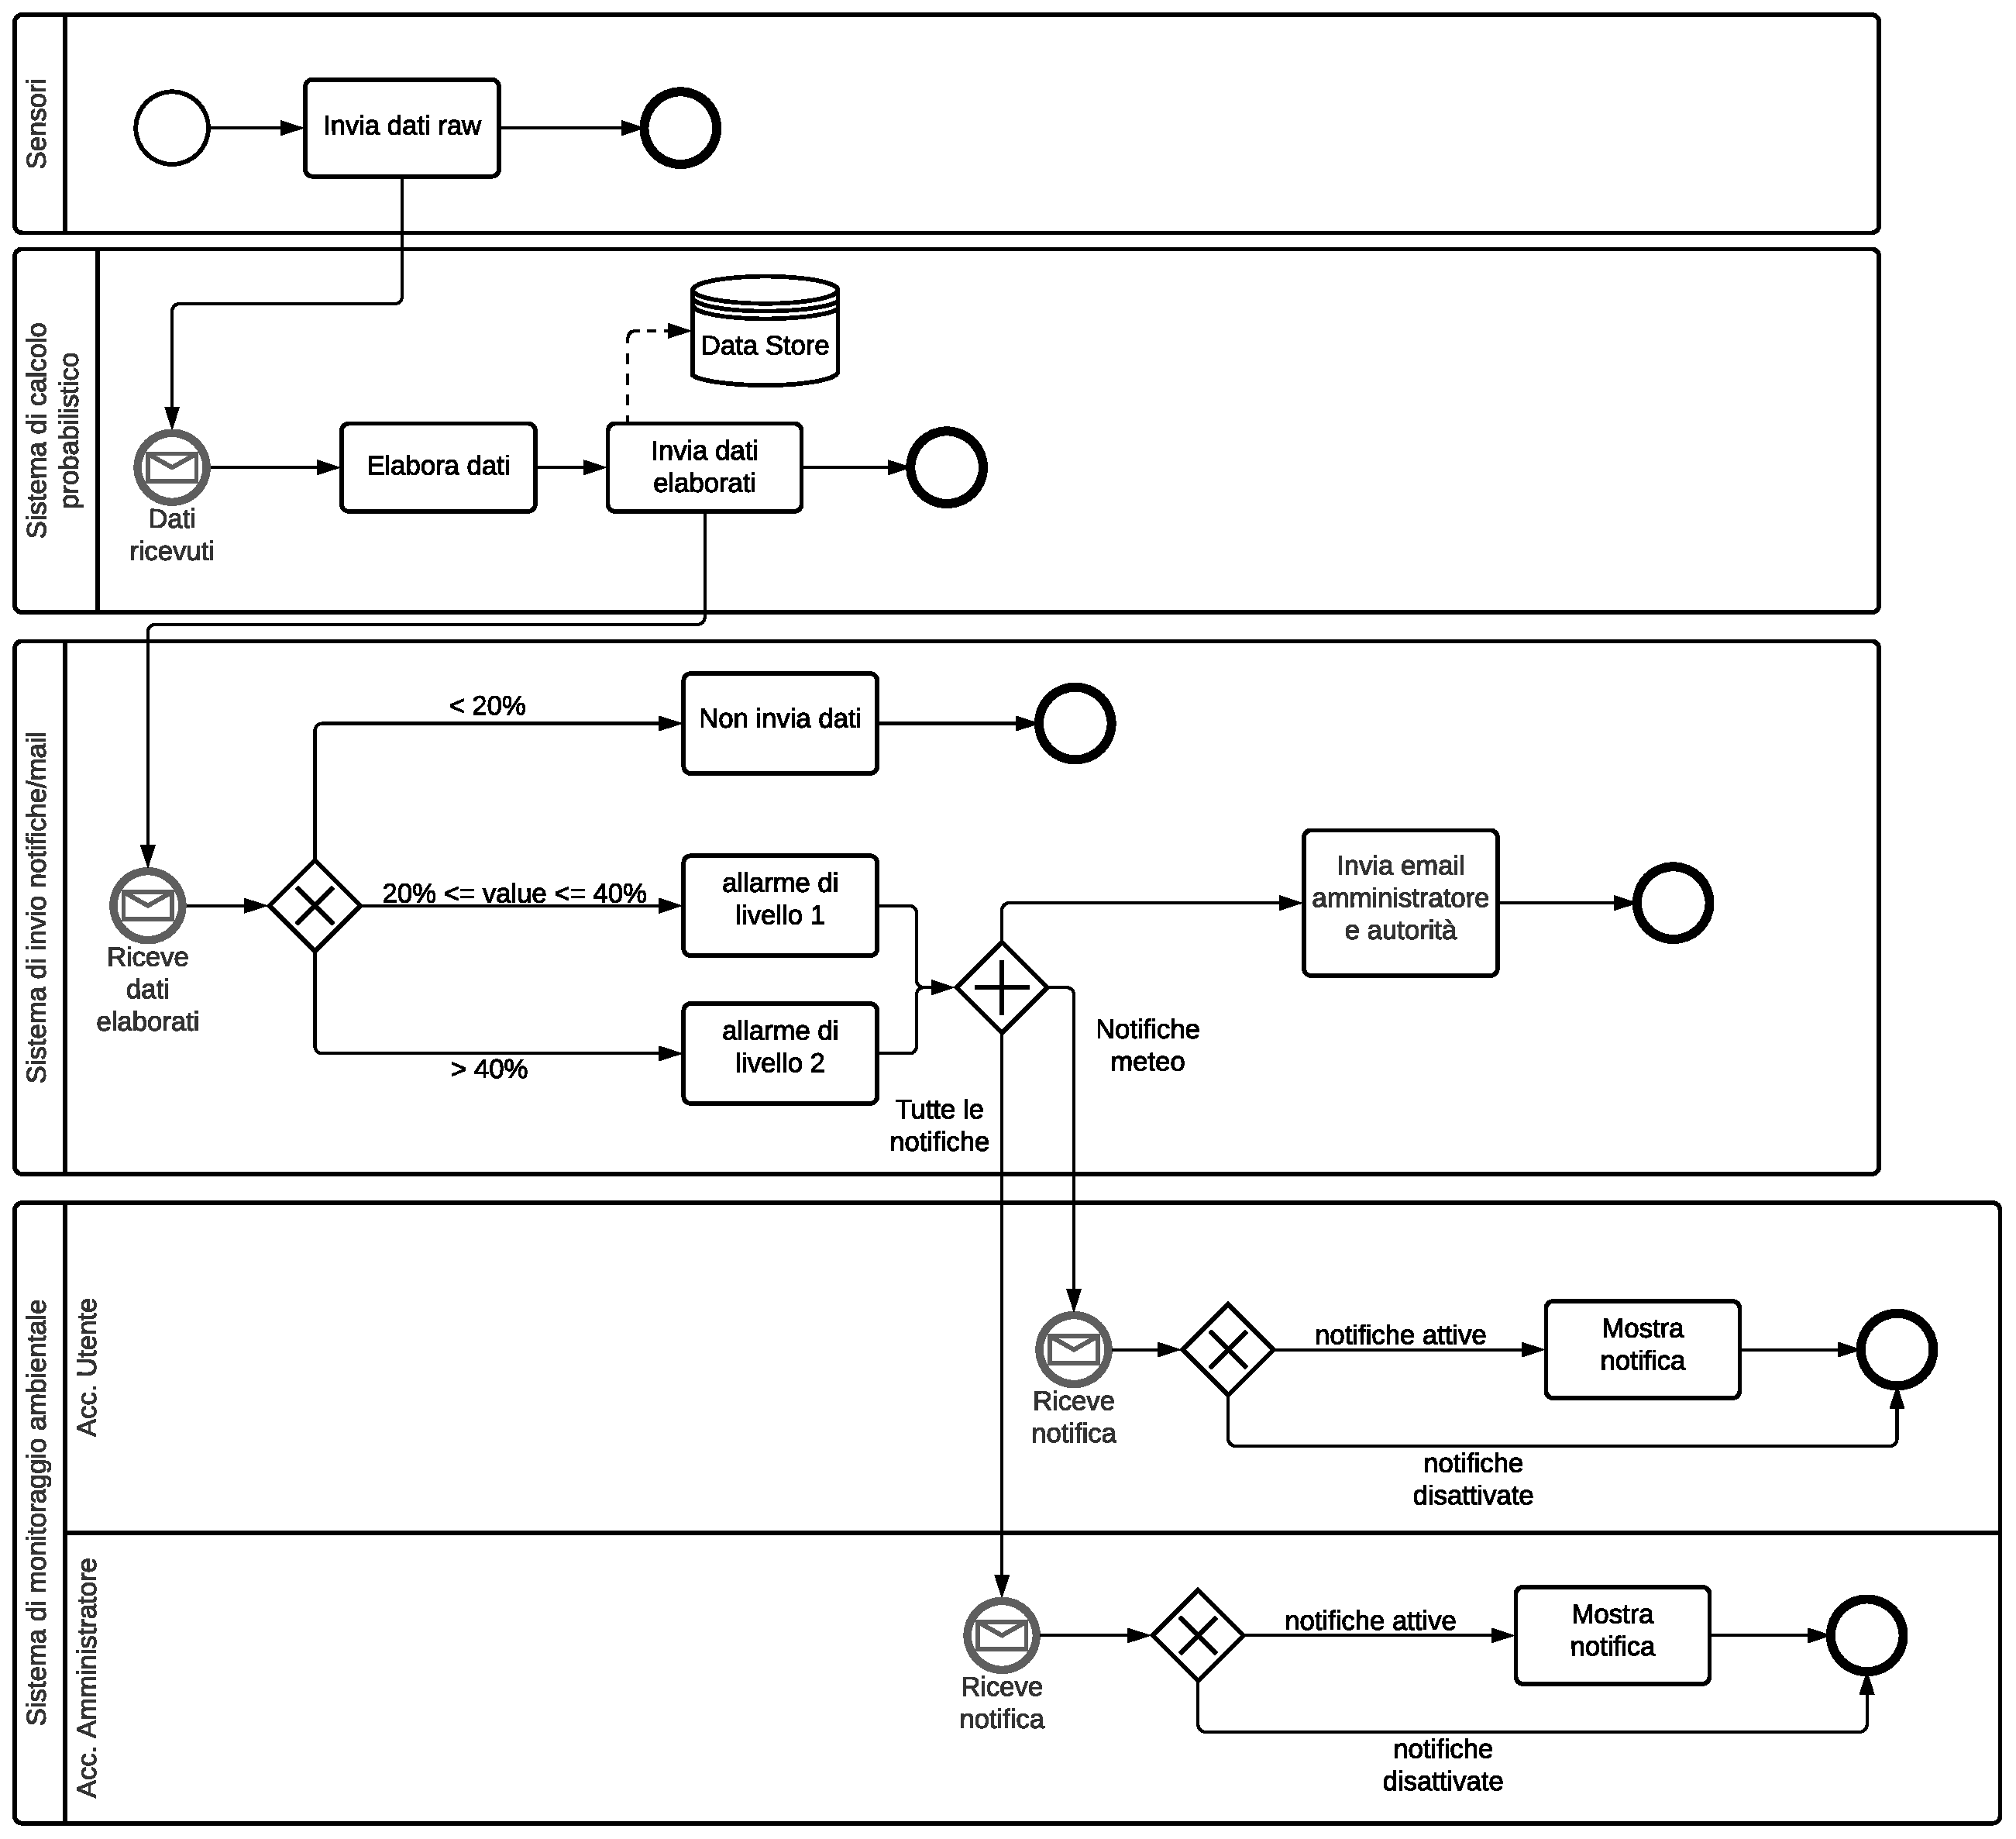
\includegraphics[scale=0.3]{Img/BPMN_Notifiche.eps}
    \caption{BPMN di invio notifiche}
    \label{fig:bpmn_notifiche}
\end{figure}

\pagebreak
\section{Livello di accoppiamento dei componenti}

\begin{table}[ht]
    \centering
    \begin{tabular}{|>{\hspace{0pt}}p{0.14\linewidth} | >{\hspace{0pt}}p{0.07\linewidth} | >{\hspace{0pt}}p{0.07\linewidth} | >{\hspace{0pt}}p{0.07\linewidth} | >{\hspace{0pt}}p{0.07\linewidth} | >{\hspace{0pt}}p{0.07\linewidth} | >{\hspace{0pt}}p{0.07\linewidth} | >{\hspace{0pt}}p{0.06\linewidth} | >{\hspace{0pt}}p{0.07\linewidth} | >{\hspace{0pt}}p{0.07\linewidth} |}
        \hline
        Accoppiamento componenti & Gestione autenticazione & Interfaccia basi di dati & Interfaccia localizzazione & Interfaccia ottenimento dati sensori & Interfaccia calcolo probabilistico & Visualizzatore menù principale & Elaboratore rischio & Interfaccia notifiche & Generatore istogrammi \\
        \hline
        Gestione autenticazione &\cellcolor{Gray} & Data & x & x & x & Data & x & x & x \\
        \hline
        Interfaccia basi di dati &\cellcolor{Gray} &\cellcolor{Gray} & Data & x & Data & Control & Data & Data & Data \\
        \hline
        Interfaccia localizzazione &\cellcolor{Gray} &\cellcolor{Gray} &\cellcolor{Gray} & x & x & x & x & x & x \\
        \hline
        Interfaccia ottenimento dati sensori &\cellcolor{Gray} &\cellcolor{Gray} &\cellcolor{Gray} &\cellcolor{Gray} & Data & x & x & x & x \\
        \hline
        Interfaccia calcolo probabilistico &\cellcolor{Gray} &\cellcolor{Gray} &\cellcolor{Gray} &\cellcolor{Gray} &\cellcolor{Gray} & x & x & x & x \\
        \hline
        \rowcolor{Gray}
        \cellcolor{white}Visualizzatore menù principale & & & & & & &\cellcolor{white} x &\cellcolor{white} x & \cellcolor{white} Data \\
        \hline
        \rowcolor{Gray}
        \cellcolor{white}Elaboratore rischio & & & & & & & &\cellcolor{white} Data  & \cellcolor{white} x \\
        \hline
        \rowcolor{Gray}
        \cellcolor{white}Interfaccia notifiche & & & & & & & & & \cellcolor{white} x \\
        \hline
        \rowcolor{Gray}
        \cellcolor{white}Generatore istogrammi & & & & & & & & &  \\
        \hline
    \end{tabular}
\end{table}

\subsection{Discussione livello di accoppiamento dei componenti}

\subsubsection*{Gestione autenticazione - Interfaccia basi di dati - Data level}
\underline{Spiegazione:} I moduli si scambiano dati riguardo l'autenticazione, ossia username e password.

\subsubsection*{Gestione autenticazione - Visualizzatore menù principale - Data level}
\underline{Spiegazione:} Il componente gestione autenticazione controlla l'autenticità delle credenziali e invia la conferma al visualizzatore menù principale.

\subsubsection*{Interfaccia base di dati - Interfaccia localizzazione - Data level}
\underline{Spiegazione:} L'interfaccia base di dati riceve i dati sulla posizione e il numero degli animali dall'interfaccia localizzazione.

\subsubsection*{Interfaccia base di dati - Interfaccia calcolo probabilistico - Data level}
\underline{Spiegazione:} L'interfaccia base di dati riceve i dati elaborati tramite l'interfaccia di calcolo probabilistico.

\subsubsection*{Interfaccia base di dati - Visualizzatore menù principale - Control level}
\underline{Spiegazione:} Il modulo visualizzatore menù principale richiede all'interfaccia base di dati le informazioni di cui necessita per visualizzare la pagina richiesta dall'utente.

\subsubsection*{Interfaccia base di dati - Elaboratore rischio - Data level}
\underline{Spiegazione:} L'interfaccia base di dati fornisce all'elaboratore di rischio i dati probabilizzati. 

\subsubsection*{Interfaccia base di dati - Interfaccia notifiche - Data level}
\underline{Spiegazione:} L'interfaccia base di dati fornisce all'interfaccia notifiche l'elenco completo di utenti e dispositivi che utilizzano l'applicazione.

\subsubsection*{Interfaccia basi di dati - Generatore istogrammi - Data level}
\underline{Spiegazione:} L'interfaccia base di dati fornisce al generatore istogrammi la posizione ed il numero degli animali richiesti.

\subsubsection*{Interfaccia ottenimento dati sensori - Interfaccia calcolo probabilistico - Data level}
\underline{Spiegazione:} L'interfaccia ottenimento dati sensori fornisce i dati grezzi rilevati dai sensori all'interfaccia di calcolo probabilistico.

\subsection*{Visualizzatore menù principale - Generatore istogrammi - Data level}
\underline{Spiegazione:} Il visualizzatore menù principale riceve l'istogramma dal generatore istogrammi.

\subsubsection*{Elaboratore rischio - Interfaccia notifiche - Data level}
\underline{Spiegazione:} Il modulo elaboratore di rischio fornisce all'interfaccia notifiche il livello di allarme calcolato.

